%\documentclass[handout,xcolor=pdftex,dvipsnames,table]{beamer}
%\documentclass[xcolor=pdftex,dvipsnames,table]{beamer}
%\documentclass{beamer}
\documentclass[11pt, xelatex]{beamer}
\definecolor{KUcrimson}{RGB}{137,32,52}
\definecolor{forestgreen}{RGB}{221,241,217}

%%==================================================================
\mode<presentation>
{
	\usetheme{AnnArbor}
	\usecolortheme{spruce}
%	\usetheme{Hannover}
%	\usetheme{Dresden}
%	\usecolortheme[named=KUcrimson]{structure} 
%	\usefonttheme[onlymath]{serif}
%	\usefonttheme{serif}
%	\useoutertheme{infolines}
%	\setbeamercovered{transparent}
}
%%==================================================================
\setbeamertemplate{footline}[frame number]
%%==================================================================
%\usepackage[english]{babel}
%\usepackage[latin1]{inputenc}
%\usepackage{times}
%\usepackage[T1]{fontenc}
%\usepackage{color,colortbl,xcolor}
%\usepackage[cjk,hangul,usecjkt1font]{kotex}
%\usepackage{pxfonts}
\usepackage{alltt}
\usepackage{natbib}
\usepackage{booktabs}
\usepackage{hyperref}
\usepackage{subfigure}
\usepackage{rotating}
\usepackage{multirow}
%\usepackage{movie15}
\usepackage{graphicx,graphics}
\usepackage{biblatex}
\usepackage{amsmath,amsfonts,amssymb,array,tabularx,theorem,epsfig}
\usepackage{listings}
\usepackage{verbatim}
%\DeclareGraphicsExtensions{.pdf,.png,.jpg}
% Set up some colors
\definecolor{myblue}{rgb}{0.14,0.11,0.49}
\definecolor{myred}{rgb}{0.74,0.22,0.15}
\definecolor{mygreen}{rgb}{0.05,0.52,0.42}
\definecolor{myyellow}{rgb}{0.96,0.92,0.13}
\definecolor{myorange}{rgb}{1,0.61,0.36}
\definecolor{mypurple}{rgb}{0.71,0.02,1}
\definecolor{mygray}{gray}{0.95}
\bibliographystyle{abbrvnat}

%%==================================================================
\newcommand{\indep}{\mathrel{\text{\scalebox{1.07}{$\perp\mkern-10mu\perp$}}}}
\newcommand{\bfPsi}{\mbox{\boldmath$\Psi$}}
\newcommand{\bfSigma}{\mbox{\boldmath$\Sigma$}}
\newcommand{\bfPhi}{\mbox{\boldmath$\Phi$}}
\newcommand{\bfLambda}{\mbox{\boldmath$\Lambda$}}
\newcommand{\bfepsilon}{\mbox{\boldmath$\epsilon$}}
\newcommand{\bfpi}{\mbox{\boldmath$\pi$}}
\newcommand{\bflambda}{\mbox{\boldmath$\lambda$}}
\newcommand{\bfbeta}{\mbox{\boldmath$\beta$}}
\newcommand{\bftheta}{\mbox{\boldmath$\theta$}}
\newcommand{\bfalpha}{\mbox{\boldmath$\alpha$}}
\newcommand{\bfzeta}{\mbox{\boldmath$\zeta$}}
\newcommand{\bfdelta}{\mbox{\boldmath$\delta$}}
\newcommand{\bfmu}{\mbox{\boldmath$\mu$}}
\newcommand{\bfxi}{\mbox{\boldmath$\xi$}}
\newcommand{\bfx}{\mbox{\boldmath$x_i$}}
\newcommand{\bfeta}{\mbox{\boldmath$\eta$}}
\newcommand{\bfrho}{\mbox{\boldmath$\rho$}}
\newcommand{\bfomega}{\mbox{\boldmath$\omega$}}
\newcommand{\benu}{\begin{enumerate}}
	\newcommand{\eenu}{\end{enumerate}}
\newcommand{\bi}{\begin{itemize}}
	\newcommand{\ei}{\end{itemize}}
\newcommand{\beq}{\begin{align*}}
\newcommand{\eeq}{\end{align*}}
\newcommand{\ci}{\perp\!\!\!\perp}
\newcommand{\pr}{\textsf{Pr}}
\newcommand{\var}{\textsf{var}}
\newcommand{\minn}{\textsf{min}}
\newcommand{\maxx}{\textsf{Max}}
\newcommand{\argmin}{\textsf{argmin}}
\newcommand{\argmax}{\textsf{argmax}}
\newcommand{\ve}{\varepsilon}
\newcommand{\bfZ}{\mbox{\boldmath$Z$}}
\newcommand{\bfr}{\mbox{\boldmath$r$}}
\newsavebox\FrameBox
\newenvironment{Frame}{%
	\par\setbox\FrameBox\hbox\bgroup\minipage{0.9\textwidth}\parskip\baselineskip\ignorespaces
}{%
	\endminipage\egroup\fbox{\box\FrameBox}\par
}

%%==================================================================
\title[] % (optional, use only with long paper titles) \h
{\textbf{GitHub \& Git overview}}

%\subtitle
%{for brief understanding on } % (optional)

\author[Hyunjun, LEE] % (optional, use only with lots of authors)
{Hyunjun, LEE}%\inst{1} \and S.~Another\inst{2}}
% - Use the \inst{?} command only if the authors have different
%   affiliation.

\institute[Korea University] % (optional, but mostly needed)
{
	%\inst{1}%
	Department of Statistics\\ \vspace{.1cm}
	Korea University}
%\and
%\inst{2}%
%Department of Theoretical Philosophy\\
%University of Elsewhere}
% - Use the \inst command only if there are several affiliations.
% - Keep it simple, no one is interested in your street address.

\date{Aug.19, 2019}

\subject{Talks}
% This is only inserted into the PDF information catalog. Can be left
% out. 

% If you have a file called "university-logo-filename.xxx", where xxx
% is a graphic format that can be processed by latex or pdflatex,
% resp., then you can add a logo as follows:
%\logo{\includegraphics[viewport= 4800 100 5000 200, scale=0.07]{../../../../LOGO/ku.jpg}}

% Delete this, if you do not want the table of contents to pop up at
% the beginning of each subsection:
%\AtBeginSubsection[]
%{
%  \begin{frame}<beamer>{Outline}
%    \tableofcontents[currentsection,currentsubsection]
%  \end{frame}
%}

% If you wish to uncover everything in a step-wise fashion, uncomment
% the following command: 
%\beamerdefaultoverlayspecification{<+->}
\renewcommand{\baselinestretch}{1.2}




%======================= document start ====================================
\begin{document}
	%\sffamily
%======================= title page ====================================
\begin{frame}
	\titlepage
\end{frame}
%=============== table of contents (based on sections) ===============
\begin{frame}{Outline}
	\tableofcontents
\end{frame}



%========================== section 1  ===================================
\section{GitHub as a personal storage (Naive approach)}
\begin{frame}
\Large
\centering
\textbf{GitHub as a personal storage (Naive approach)}
\end{frame}
%------------ creating a new repository -----------------
\begin{frame}{Creating a new repository}
\bi
\item User can make new repository(folder) after creating new GitHub account \\ by click on  "Create a repository" or "New" buttons
\ei
\begin{figure}
	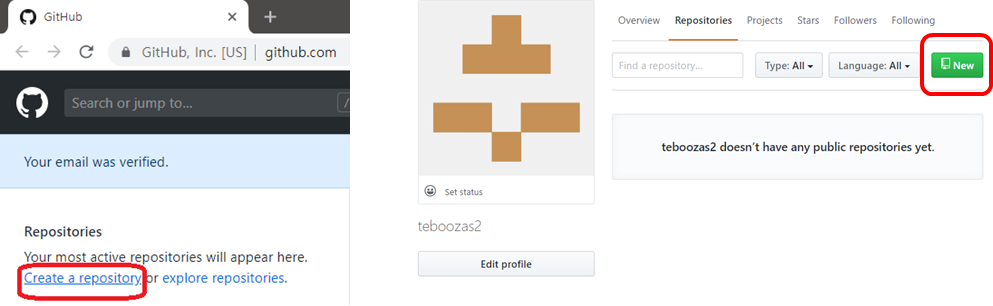
\includegraphics[width=0.8\textwidth]{lab_seminar/lab_seminar(GitHub_Git)/images/create_new_repo.png}
	\inclue
	\caption{two ways to create new repository}
\end{figure}
\end{frame}

\begin{frame}{Creating a new repository}
\bi
\item Name of a repository is url as well (need to be careful)
\item Filling out README file and description details are recommended
\ei
\begin{figure}
	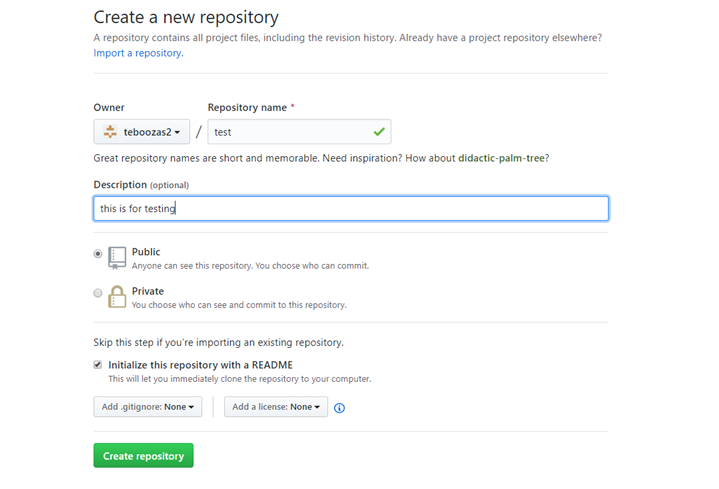
\includegraphics[width=0.6\textwidth]{lab_seminar/lab_seminar(GitHub_Git)/images/create_new_repo_2.png}
	\inclue
	\caption{options for creating a new repository}
\end{figure}
\end{frame}

\begin{frame}{Creating a new repository}
\begin{figure}
	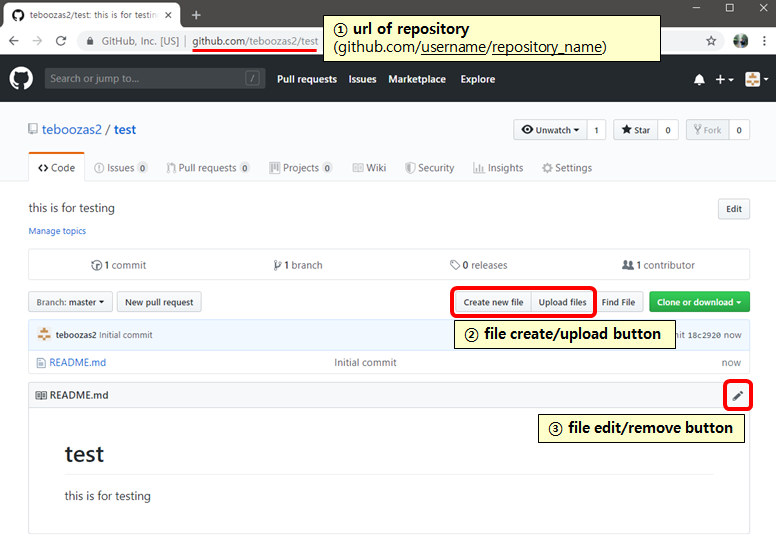
\includegraphics[width=0.7\textwidth]{lab_seminar/lab_seminar(GitHub_Git)/images/create_new_repo_3.png}
	\inclue
	\caption{initial settings of a new repository}
\end{figure}
\end{frame}

%------------ add, edit, remove files -----------------
\begin{frame}{Upload, edit, and remove files}
\bi
\item To add files to repo, click "Upload files" 
\item Users can add items with drag up or to choose them manually
\item Filling out commit message is strongly recommended
\item After write down all messages, click "commit changes" to save files\\
(we will check later what "commit" means)
\ei
\end{frame}

\begin{frame}{Upload, edit, and remove files}
\begin{figure}
	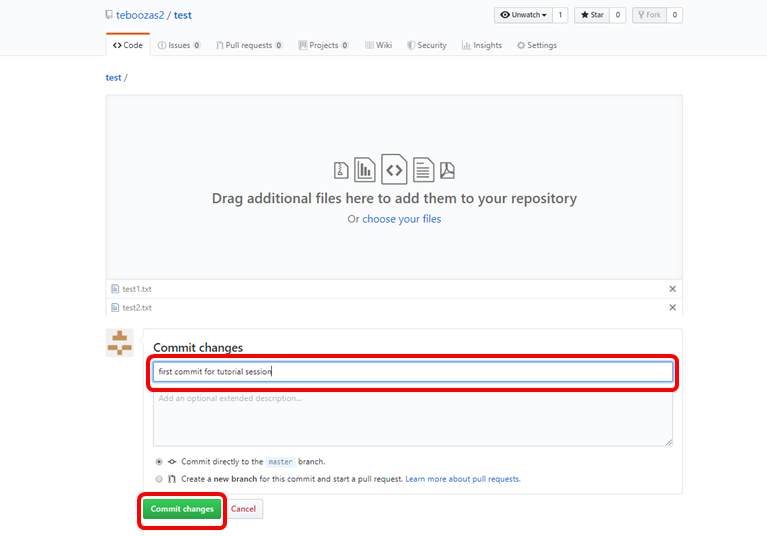
\includegraphics[width=0.7\textwidth]{lab_seminar/lab_seminar(GitHub_Git)/images/add_edit_remove_1.png}
	\caption{two text files are being uploaded}
\end{figure}
\end{frame}

\begin{frame}{Upload, edit, and remove files}
\begin{figure}
	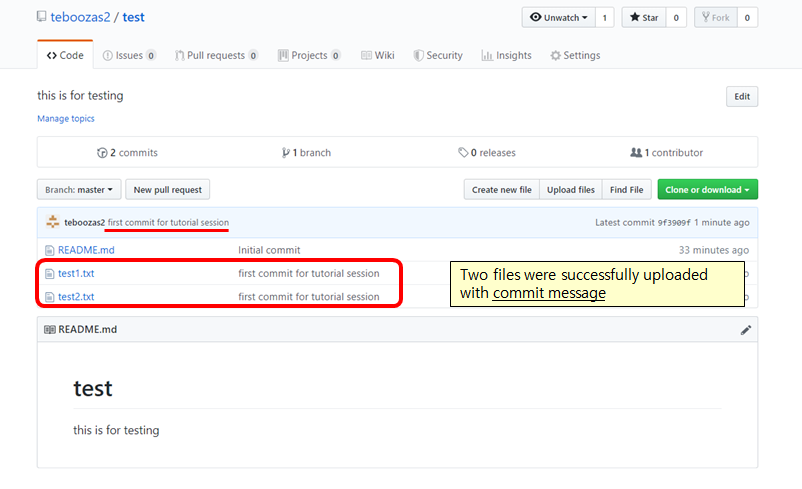
\includegraphics[width=0.7\textwidth]{lab_seminar/lab_seminar(GitHub_Git)/images/add_edit_remove_2.png}
	\caption{files were successfully uploaded with commit message}
\end{figure}
\end{frame}

\begin{frame}{Upload, edit, and remove files}
\bi
\item Users can edit code or texts in repo directly on GitHub\\(not frequently used)
\ei
\begin{figure}
	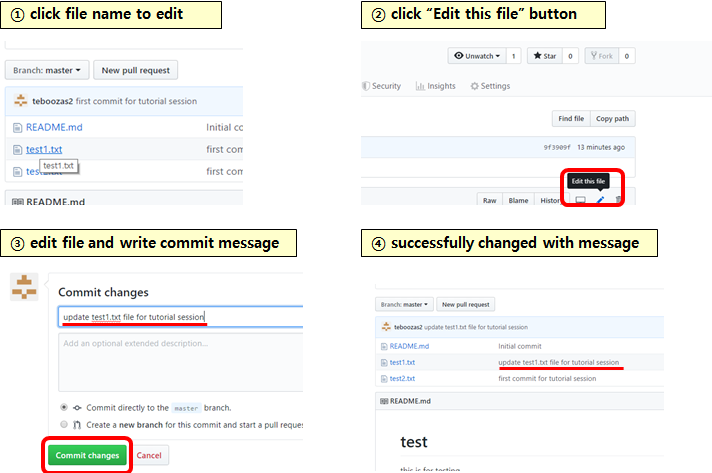
\includegraphics[width=0.6\textwidth]{lab_seminar/lab_seminar(GitHub_Git)/images/add_edit_remove_3.png}
	\caption{workflow editing files on GitHub}
\end{figure}
\end{frame}

\begin{frame}{Upload, edit, and remove files}
\bi
\item Users can delete a file similarly with editing
\ei
\begin{figure}
	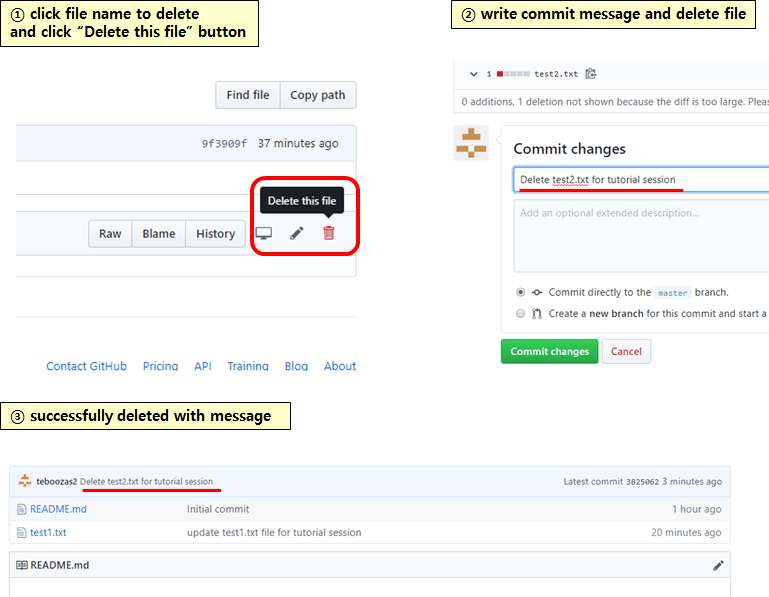
\includegraphics[width=0.6\textwidth]{lab_seminar/lab_seminar(GitHub_Git)/images/add_edit_remove_4.png}
	\caption{workflow deleting files on GitHub}
\end{figure}
\end{frame}

%------------ more on repository -----------------
\begin{frame}{More on GitHub repository}
\bi
\item rename, ownership transfer, removal of repository can be done\\in "settings"
\item Changing histories of repository are all recorded and perfectly re-accessible
    \bi
    \item[-] Files that edited and removed are preserved in each commit status
    \item[-] That's why commit messages are so important\\
    (to track records and access previous status of files if needed)
    \ei
\item Re-accessibility to previous status is powerful feature of Git\\(and GitHub itself)
\item Although repo has no storage limit, maintaining it light is desirable
\\(using local machine or cloud storage are better for large data)
\ei
\end{frame}

\begin{frame}{More on GitHub repository}
\begin{figure}
	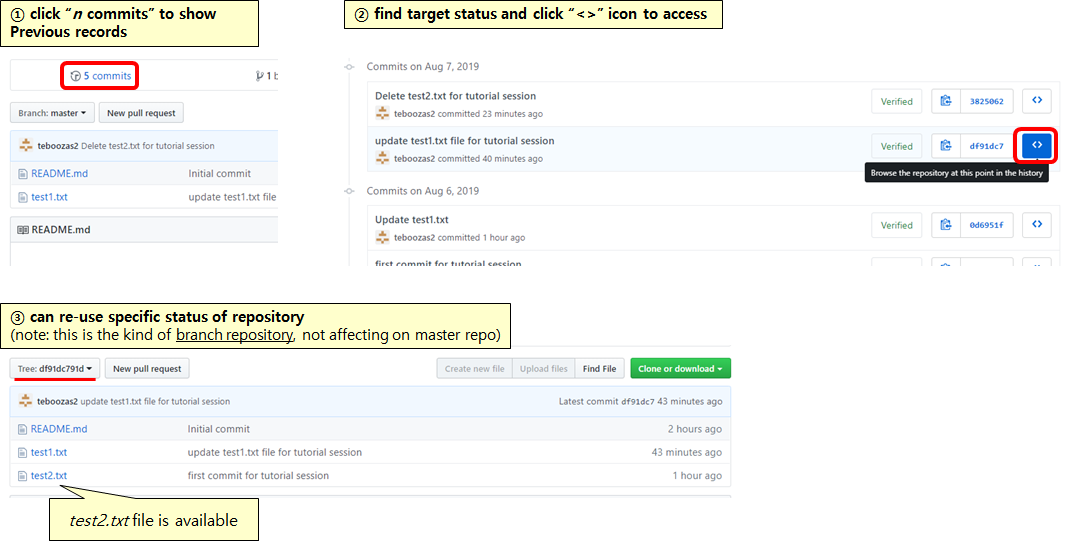
\includegraphics[width=0.8\textwidth]{lab_seminar/lab_seminar(GitHub_Git)/images/more_on_repo_1.png}
	\caption{workflow accessing previous status of repo}
\end{figure}
\end{frame}

\begin{frame}{More on GitHub repository}
\bi
\item What have been covered are enough for personal use\\and portfolio of own works
\item However, GitHub is essentially the collaborative tool for developers\\
based on Git software and Git repository
\item For rich and interactive use of GitHub, understanding Git and its characteristic workflow is required
\ei
\end{frame}




%========================== section 2  ===================================
\section{Quick Git - handling local repository}
\begin{frame}
\Large
\centering
\textbf{Quick Git - handling local repository}
\end{frame}

%------------ What is Git? -----------------
\begin{frame}{What is Git?}
\bi
\item Git is a version control system(VCS)
    \bi
    \item[-] A version control system \textbf{records changes} to a file and files(folder)
    \item[-] Tracking records of files is useful for large scale collaboration
    \ei
\item Git is the most common VCS due to its speed, efficiency,\\and immensely large web hosting service, the GitHub
\ei
\begin{figure}
	
\includegraphics[width=0.8\textwidth]{lab_seminar/lab_seminar(GitHub_Git)/images/what_is_git_1.png}
\end{figure}
\end{frame}

\begin{frame}{What is Git?}
\bi
\item Git takes 'snapshots' of status and records them
    \bi
    \item[-] Most of VCSs track every single file change individually
    \item[-] In contrast, Git stores whole changes of folder into a small size of snapshot containing links of files
    \ei
\item Git has 3 main states of files (which is called 'tracked status')
    \bi
    \item[-] \textbf{modified}: files in tracked status have been revised, not recorded
    \item[-] \textbf{staged}: modified files are on 'stage', ready to be recorded
    \item[-] \textbf{committed}: staged files are recorded into a snapshot \textbf{\color{red}{with checkpoint}}
    \item[-] Note that not every files in Git repo are in committed state\\
    (untracked, modified, staged files don't have snapshots)
    \ei
\ei
\end{frame}

\begin{frame}{What is Git?}
\begin{figure}
	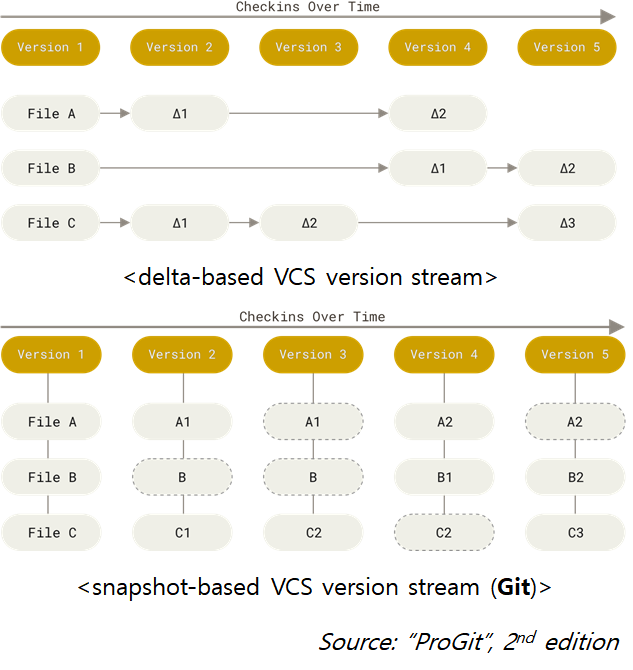
\includegraphics[width=0.55\textwidth]{lab_seminar/lab_seminar(GitHub_Git)/images/what_is_git_2.png}
\end{figure}
\end{frame}


%------------ Lifecycle of Git -----------------
\begin{frame}{Lifecycle of Git}
\bi
\item Summary of Git lifecycle(workflow) is depicted below
    \bi
    \item[-] tracked status: unmodified(\textbf{committed}), modified, staged states
    \item[-] untracked status: files in local folder, but not be tracked by Git
    \ei
\ei
\begin{figure}
	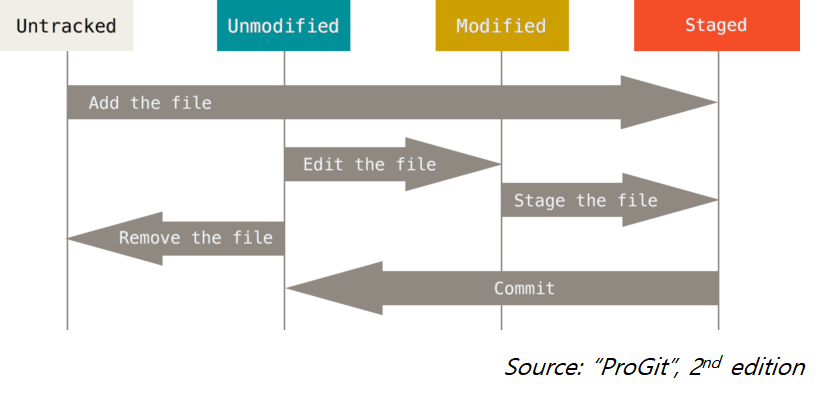
\includegraphics[width=0.8\textwidth]{lab_seminar/lab_seminar(GitHub_Git)/images/lifecycle_of_Git.png}
\end{figure}
\end{frame}

%------------ Basic commands for Git CLI -----------------
\begin{frame}{Basic commands for Git CLI}
\bi
\item Most common tool for handling Git on local machine is CLI
    \bi
    \item[-] CLI(Command-Line Interface) includes Git bash(Windows), Terminal(Mac), UNIX/LINUX shell prompt, etc.
    \ei
\item Users can use Git with CLI after installing Git on own machine\\
(you can get Git from here: \url{https://git-scm.com/downloads})
\ei
\begin{figure}
	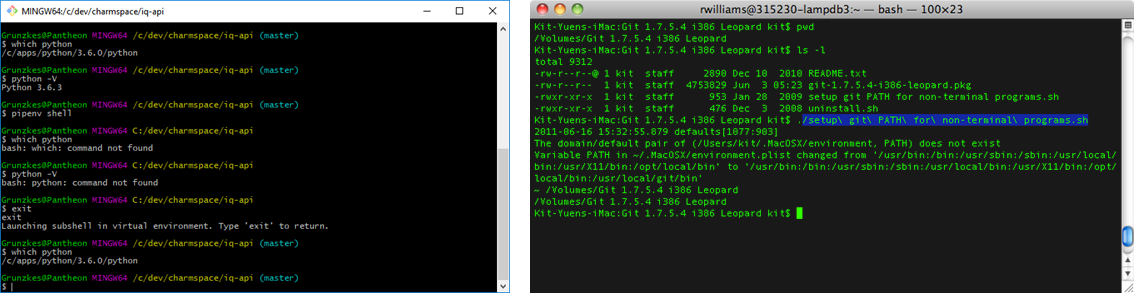
\includegraphics[width=0.8\textwidth]{lab_seminar/lab_seminar(GitHub_Git)/images/commands_basic_1.png}
	\caption{example of CLI}
\end{figure}
\end{frame}

\begin{frame}{Basic commands for Git CLI}
\bi
\item After run CLI w.r.t types of machine, handling Git can be done\\with this basic form of command statement: 
\ei
\centering\colorbox{myyellow}{\verb|git <command> (options)}
\bi
\item Important commands can be categorized as below:
    \bi
    \item[-] configuration \& settings - \colorbox{mygray}{\verb|config}, \colorbox{mygray}{\verb|help}
    \item[-] making a Git repository - \colorbox{mygray}{\verb|init}, \colorbox{mygray}{\verb|clone}
    \item[-] snapshot handling - \colorbox{mygray}{\verb|add}, \colorbox{mygray}{\verb|status}, \colorbox{mygray}{\verb|commit}
    \item[-] branching - \colorbox{mygray}{\verb|branch}, \colorbox{mygray}{\verb|checkout}, \colorbox{mygray}{\verb|merge}
    \item[-] sharing projects - \colorbox{mygray}{\verb|remote}, \colorbox{mygray}{\verb|fetch}, \colorbox{mygray}{\verb|pull}, \colorbox{mygray}{\verb|push}
    \ei
\item first three categories will be covered in this section\\(and remainders for later sections)
\ei
\end{frame}

%------------ Basic commands for Git CLI - configuration & settings -----------------
\begin{frame}{Basic commands for Git CLI - \textbf{configuration \& settings}}
\bi
\item \colorbox{mygray}{\verb|config} command (examples)
    \bi
    \item[-] command for configuration, including user information, etc.
    \item[-] \colorbox{mygray}{\verb|git config --global user.name "John"}:\\set user name as 'John'
    \item[-] \colorbox{mygray}{\verb|git config --global user.email john@example.com}:\\set user e-mail as 'john@example.com'
    \item[-] \colorbox{mygray}{\verb|git config --list}: check global settings of local Git
    \ei
\item \colorbox{mygray}{\verb|help} command (examples)
    \bi
    \item[-] roughly two ways to get help for sepcific command
    \item[-] \colorbox{mygray}{\verb|git help config}:\\get the manpage help for the \colorbox{mygray}{\verb|config} command
    \item[-] \colorbox{mygray}{\verb|git add -h}:\\git summary help for the \colorbox{mygray}{\verb|add} command directly from the kernel
    \ei
\ei
\end{frame}

%------------ Basic commands for Git CLI - making a Git repository -----------------
\begin{frame}{Basic commands for Git CLI - \textbf{making a Git repository}}
\bi
\item \colorbox{mygray}{\verb|init} command
    \bi
    \item[-] turn current directory(folder) which CLI is running on, into a\\Git repository (can store snapshots)
    \item[-] \colorbox{mygray}{\verb|git init} (just simply enter it!)
    \ei
\item \colorbox{mygray}{\verb|clone} command
    \bi
    \item[-] get a clone(copy) of existing Git repository, including all of the\\previous snapshots
    \item[-] \colorbox{mygray}{\verb|git clone https://github.com/John/myrepo Johnrepo}:\\copy Git repo 'myrepo' from url, and change its name into 'Johnrepo'
    \item[-] \colorbox{mygray}{\verb|git clone} is useful statement, especially for Google Colab
    \ei
\ei
\end{frame}

%------------ Basic commands for Git CLI - snapshot handling  -----------------
\begin{frame}{Basic commands for Git CLI - \textbf{snapshot handling}}
\bi
\item \colorbox{mygray}{\verb|add} command (examples)
    \bi
    \item[-] turn modified \& untracked files into staged files
    \item[-] \colorbox{mygray}{\verb|git add README.txt}:\\send 'README.txt' file(untracked or modified) to staged state
    \item[-] \colorbox{mygray}{\verb|git add -A}:\\send all of the untracked/modified files in Git repo to staged state
    \ei
\item \colorbox{mygray}{\verb|status} command (examples)
    \bi
    \item[-] get a view of states of all files in Git repo (including untracked ones)
    \item[-] \colorbox{mygray}{\verb|git status}: return list of files by states in the repo
    \item[-] \colorbox{mygray}{\verb|git status -s}: return short version of status
    \ei
\ei
\end{frame}

\begin{frame}{Basic commands for Git CLI - \textbf{snapshot handling}}
\bi
\item \colorbox{mygray}{\verb|commit} command (examples)
    \bi
    \item[-] take a snapshot of status of Git repo and store it with a checkpoint
    \item[-] \colorbox{mygray}{\verb|git commit -m "initial commit"}:\\take a snapshot of status with commit message 'initial commit'
    \item[-] \colorbox{mygray}{\verb|git commit -a -m 'second commit'}:\\take a snapshot of status with commit message 'second commit',\\skipping staging step (untracked/modified files are automatically committed without \colorbox{mygray}{\verb|add} command)
    \ei
\item Notes on \colorbox{mygray}{\verb|commit}
    \bi
    \item[-] After running \colorbox{mygray}{\verb|commit} command, all committed files are turned into unmodified state (recall 'the lifecycle of Git')
    \item[-] Every commits have their own checkpoint, called 'SHA-1 checksum'\\(looks like \colorbox{mygray}{\verb|3c163a0})
    \item[-] Users can revert to or compare snapshots with checkpoints
    \ei
\ei
\end{frame}

%------------ Notes on basic commands for Git CLI -----------------
\begin{frame}{Notes on basic commands for Git CLI}
\bi
\item If you were confused, recall the depiction of 'the lifecycle of Git'
\item Although there are lots of commands and options, \colorbox{mygray}{\verb|add} and \colorbox{mygray}{\verb|commit} are the fundamental ones
\item Past checkpoints of commit contains all files at the time, even  they were deleted and do not exist now on (very useful for recovery)
\item The reason why Git separates states into 'staged' and 'unstaged' \\is that, users can record changes 'as the way of project'\\(rather than save every single changes of each files)
\ei
\end{frame}




%========================== section 3  ===================================
\section{Quick Git - branching}
\begin{frame}
\Large
\centering
\textbf{Quick Git - branching}
\end{frame}

%------------ What is branching -----------------
\begin{frame}{What is branching?}
\bi
\item Branching method allows running independent subprojects
    \bi
    \item Developers can work independently(debugging, add functionality, etc.) without concern of conflicts exploiting branches
    \item Branching is the core of DVCS(Distributed VCS) for massive collaborative projects
    \ei
\item Branching of Git is easy and fast enough to be beloved
\ei
\begin{figure}
	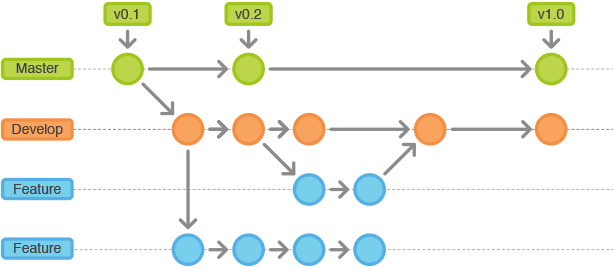
\includegraphics[width=0.55\textwidth]{lab_seminar/lab_seminar(GitHub_Git)/images/what_is_branch_1.png}
	\caption{example of branching workflow}
\end{figure}
\end{frame}

\begin{frame}{What is branching?}
\bi
\item Generally, branching follows workflow below:
    \bi
    \item[1.] create branch repository with purpose from master branch
    \item[2.] move onto created branch, and do add/commit to achieve purpose
    \item[3.] after commit, move back to master branch and merge outputs of target
    \ei
\item Each step above is matched with the corresponding commands:\\\colorbox{mygray}{\verb|branch}, \colorbox{mygray}{\verb|checkout}, \colorbox{mygray}{\verb|merge}
\ei
\end{frame}

%------------ Commands for Git branching -----------------
\begin{frame}{Commands for Git branching}
\bi
\item \colorbox{mygray}{\verb|branch} command (examples)
    \bi
    \item[-] create \& list branches from the other branch (mostly 'master')
    \item[-] \colorbox{mygray}{\verb|git branch debug}: create 'debug' branch based on current branch
    \item[-] \colorbox{mygray}{\verb|git branch}: return existing branches based on current branch
    \ei
\item \colorbox{mygray}{\verb|checkout} command
    \bi
    \item[-] switch branches for working on
    \item[-] \colorbox{mygray}{\verb|git debug}: moves to 'debug' branch for working on
    \ei
\item \colorbox{mygray}{\verb|merge} command
    \bi
    \item[-] merge outputs of a branch with the other's
    \item[-] \colorbox{mygray}{\verb|git merge debug}:\\
    (automatically) combine files in current branch with files in \\'debug' branch (current $\leftarrow$ 'debug')
    \ei
\ei
\end{frame}

%------------ Notes on commands for Git branching -----------------
\begin{frame}{Notes on commands for Git branching}
\bi
\item Even though commands and their workflow seems quite simple,\\Git branching can be extended for numerous non-linear sub-projects
\item In case of conflict(fail to merge), users can fix conflict manually and commit after fixing, or using \colorbox{mygray}{\verb|mergetool} command
\item Users can review outputs in branch before merge them to master\\
$\Rightarrow$ this forms basis of 'pull requests' in GitHub service
\ei
\end{frame} 



%========================== section 4  ===================================
\section{Quick Git - sharing projects (remote repository)}
\begin{frame}
\Large
\centering
\textbf{Quick Git - sharing projects (remote repository)}
\end{frame}

%------------ remote repository and web hosting services -----------------
\begin{frame}{Remote repository and web hosting service(GitHub)}
\bi
\item Most of the projects using VCS(including Git) store files and\\commit checksums in remote repository
    \bi
    \item remote repository is usually hosted on the Internet or network
    \ei
\item There are many web hosting services providing remote repository\\and the most famous one is \textbf{GitHub}
\item Communication between local Git and web-based GitHub\\can be easily done with local CLI and its commands
\ei
\end{frame}

\begin{frame}{Remote repository and web hosting service(GitHub)}
\bi
\item workflow to control remote repo can be summarized:
    \bi
    \item[1.] add(link) or check remote repository on local machine
    \item[2.] get all data from origin remote and merge them with local data
    \item[3.] after fixing merged local data, merge them toward origin remote
    \ei
\item Each step above is matched with the corresponding commands:\\\colorbox{mygray}{\verb|remote}, \colorbox{mygray}{\verb|fetch} or \colorbox{mygray}{\verb|pull}, \colorbox{mygray}{\verb|push}
\ei
\end{frame}

%------------ Commands for controlling remote -----------------
\begin{frame}{Commands for controlling remote}
\bi
\item \colorbox{mygray}{\verb|remote} command (examples)
    \bi
    \item[-] link \& list remote(mostly called 'origin') from hosting service
    \item[-] \colorbox{mygray}{\verb|git remote add origin  https://github.com/John/myrepo}:\\add(link) remote 'origin' from given url of hosting service
    \item[-] \colorbox{mygray}{\verb|git remote}: return existing linked remote repositories
    \ei
\item \colorbox{mygray}{\verb|fetch} command (examples)
    \bi
    \item[-] get data from remote (except for things already exist)
    \item[-] \colorbox{mygray}{\verb|git fetch origin}: get data from 'origin' remote to current repo
    \ei
\ei
\end{frame}

\begin{frame}{Commands for controlling remote}
\bi
\item \colorbox{mygray}{\verb|pull} command (examples)
    \bi
    \item[-] do 'fetch' and 'merge' at the same time
    \item[-] \colorbox{mygray}{\verb|git pull origin master}:\\get data from 'origin' remote to current repo('master') and merge them within 'master'
    \ei
\item \colorbox{mygray}{\verb|push} command (examples)
    \bi
    \item[-] share local commits with the origin remote repository
    \item[-] easily can be thought as saving data from local to GitHub repository
    \item[-] \colorbox{mygray}{\verb|git push origin master}: \\share commits in 'master' repo with 'origin' remote repo
    \ei
\ei
\end{frame}


%------------ Notes on commands for controlling remote -----------------
\begin{frame}{Notes on commands for controlling remote}
\bi
\item \colorbox{mygray}{\verb|pull} and \colorbox{mygray}{\verb|push} are key commands for open-source projects
    \bi
    \item These two commands allow interactive workflow between local\\and remote repository
    \item Combining with branching, \colorbox{mygray}{\verb|pull} and \colorbox{mygray}{\verb|push} commands become\\more powerful
    \ei
\item \colorbox{mygray}{\verb|clone} versus \colorbox{mygray}{\verb|remote add}
    \bi
    \item \colorbox{mygray}{\verb|clone} command get entire repository into local machine, but this copied repo is not linked with origin remote
    \item On the other hand, \colorbox{mygray}{\verb|remote add} command just link local machine with web-based repository, and not pull down commits and data
    \ei
\ei
\end{frame} 




%========================== section 5  ===================================
\section{GitHub as a collaborative tool for open-source projects}
\begin{frame}
\Large
\centering
\textbf{GitHub as a collaborative tool\\for open-source projects}
\end{frame}

%------------ Review: snapshotting, branching, and remote control -----------------
\begin{frame}{Review: snapshotting, branching, and remote control}
\bi
\item Combining all, working on a Git project can be summarized:
    \bi
    \item[1.]create a project on GitHub repository
    \item[2.]make a Git repository on local machine for maintenance of the project\\- \colorbox{mygray}{\verb|init}, \colorbox{mygray}{\verb|clone}
    \item[3.]connect local repository with remote GitHub project repository\\- \colorbox{mygray}{\verb|remote}
    \item[4.]get previous commits from remote repository\\- \colorbox{mygray}{\verb|fetch} or \colorbox{mygray}{\verb|pull}
    \item[5.]develop(snapshot) a project on local with related commits from remote\\- \colorbox{mygray}{\verb|add}, \colorbox{mygray}{\verb|status}, \colorbox{mygray}{\verb|commit}
    \item[6.]share additional commits from local to Github repository\\- \colorbox{mygray}{\verb|push}
    \item[7.]if needed, use branching for independent works\\- \colorbox{mygray}{\verb|branch}, \colorbox{mygray}{\verb|checkout}, \colorbox{mygray}{\verb|merge}
    \ei
\ei
\end{frame}

\begin{frame}{Working on a open-source projects}
\bi
\item As mentioned before, GitHub is widely applied on large number of open-source projects
\item Thus, GitHub provides functionality for teamwork onto projects owned by group of users, as well as for potential contributors
\item For this, GitHub came up with the concept of \textbf{Pull Request}
\ei
\begin{figure}
	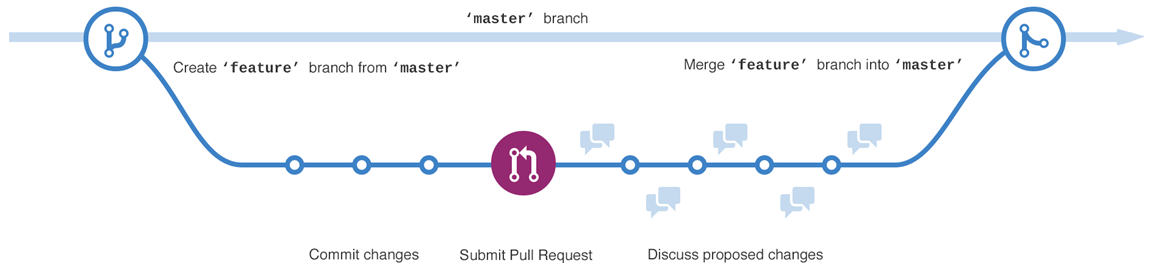
\includegraphics[width=0.85\textwidth]{lab_seminar/lab_seminar(GitHub_Git)/images/working_on_open_1.png}
	\caption{standard GitHub workflow}
\end{figure}
\end{frame}

\begin{frame}{Working on a open-source projects}
\bi
\item If someone wants to contribute to a open-source project via GitHub, followings are the standard steps
    \bi
    \item[1.]\textbf{Fork} target GitHub project into personal account
    \item[2.]clone and link(remote) it to own local machine using CLI
    \item[3.]create a new branch to work with
    \item[4.]add commits to contribute to the project (still on a branch)
    \item[5.]push commits in branch toward origin remote (not to master branch)
    \item[6.]click \textbf{Compare \& pull request} button to submit pull request
    \item[7.]project owners will review and discuss upon pull requests,\\
    and decide whether to merge this pull request or not
    \item[8.]if accepted, project owners will merge commits in the pull request
    \item[9.]pull updated project into local repo and delete previous branch
    \item[10.]repeat 3. to 9. for additional contribution
    \ei
\ei
\end{frame}

\begin{frame}{Working on a open-source projects}
\bi
\item Shortly, \textbf{pull request} is the expression of asking to merge user's\\commits with codes in the open-source project\\
(and darely described as 'the heart of collaboration on GitHub')
\item You can be a contributor for named GitHub project with this process, including NumPy, Scikit-learn, Tensorflow, PyTorch, etc.
\ei
\end{frame}

\begin{frame}{\textbf{Conclusion}}
\bi
\item You don't have to get to know all of these at once.\\Instead, try to get used to GitHub and Git CLI (using toy examples)
\item At first, it is desirable to make a habit of managing GitHub account "regularly", even with the purpose of personal storage
\item Keep track of concepts of version control and collaborative open-source project.
It will surely be helpful to both academic achievement and successful career.
\ei
\end{frame}

\begin{frame}{Reference}
\bi
\item[-]ProGit book, 2nd edition (Chacon, Straub) \href{https://git-scm.com/book/en/v2}{(link)}
\item[-]GitHub Guides official webpages \href{https://guides.github.com/}{(link)}
\item[-]Opentutorials.org - Git from hell \href{https://opentutorials.org/course/2708}{(link)}
\item[-]Korean blogger(developer) - Pull Requests \href{https://wayhome25.github.io/git/2017/07/08/git-first-pull-request-story/}{(link)}
\ei
\end{frame}

\end{document}